%%%%%%%%%%%%%%%%%%%%%%%%%%%%%%%%%%%%%%%%%%%%%%%%%%%%%%%%%%%%%%%%%%%%%
% LaTeX Template: Project Titlepage Modified (v 0.1) by rcx
%
% Original Source: http://www.howtotex.com
% Date: February 2014
% 
% This is a title page template which be used for articles & reports.
% 
% This is the modified version of the original Latex template from
% aforementioned website.
% 
%%%%%%%%%%%%%%%%%%%%%%%%%%%%%%%%%%%%%%%%%%%%%%%%%%%%%%%%%%%%%%%%%%%%%%

\documentclass[12pt]{report}
\usepackage[a4paper]{geometry}
\usepackage[myheadings]{fullpage}
\usepackage{fancyhdr}
\usepackage{lastpage}
\usepackage{graphicx, wrapfig, subcaption, setspace, booktabs}
\usepackage[english]{babel}
\usepackage{color}
\usepackage{hyperref}
\usepackage{array}
\usepackage{supertabular}
\usepackage{hhline}
\usepackage{enumitem}
\usepackage[T1]{fontenc}
\usepackage[utf8]{inputenc}
\usepackage{graphicx}


\newcommand{\HRule}[1]{\rule{\linewidth}{#1}}
\renewcommand{\theenumii}{\arabic{enumii}.}
\addto\captionsenglish{
  \renewcommand{\contentsname}
    {Innhold}
}
\onehalfspacing
\setcounter{tocdepth}{5}
\setcounter{secnumdepth}{5}

%-------------------------------------------------------------------------------
% HEADER & FOOTER
%-------------------------------------------------------------------------------
\pagestyle{fancy}
\fancyhf{}
\setlength\headheight{15pt}
\fancyhead[L]{Team D} 
\fancyhead[R]{Universitetet i Bergen}
\fancyfoot[R]{Page \thepage\ of \pageref{LastPage}}
%-------------------------------------------------------------------------------
% TITLE PAGE
%-------------------------------------------------------------------------------

\begin{document}

\title{ \normalsize \textsc{}
		\\ [2.0cm]
		\HRule{0.5pt} \\
		\LARGE \textbf{\uppercase{Spooks}}
		\HRule{2pt} \\ [0.5cm]
		\normalsize \today \vspace*{5\baselineskip}}

\date{}

\author{
		Team D  \\ 
		Universitetet i Bergen \\
		Informatikk }

\maketitle
\tableofcontents
\newpage

%-------------------------------------------------------------------------------
% BODY
%-------------------------------------------------------------------------------

\section*{Bruksm{\o}nstertekst:}
\addcontentsline{toc}{section}{Bruks{\o}nstertekst:}
\textbf{Tittel}: Komme seg ut av huset
\bigskip \\
\textbf{Akt{\o}rer}: Spiller, Maskin 
\bigskip \\
\textbf{Prim{\ae}rakt{\o}r}: Spiller
\bigskip \\
\textbf{Tid}: Avhenger av spilleren (har spilleren spilt lignende spill tidligere/l{\o}st lignende g{\aa}ter), runder p{\aa} * minutter (avhenger av hvor avansert g{\aa}tene blir)
\bigskip \\
\textbf{M{\aa}l}: L{\o}se alle g{\aa}tene og finne alle n{\o}klene for {\aa} komme seg ut av huset
\bigskip \\
\textbf{Pre-conditions:} Spillet er startet p{\aa} en datamaskin
\bigskip \\
\textbf{Variasjons scenario}: Spilleren kan flytte seg mellom alle {\aa}pne rom, selvom dette ikke er n{\o}dvendig for m{\aa}let

\subsection*{Hovedflyt:}

\begin{enumerate}
\item Meny (Start - load game - options - quit)
\item Spiller velger {\aa} starte ett nytt spill
\item Systemet oppretter et nytt spill
\item Systemet starter en klokke som teller ned fra * minutter
\item Spiller trykker p{\aa} et objekt i spillet
\item Spiller f{\aa}r objektet
\item Systemet legger tingen i Spillerens inventory
\end{enumerate}

\textit{Steg 4-7 g{\aa}r i loop til Spiller har riktig objekt (evt. l{\o}st en g{\aa}te) til {\aa} g{\aa} videre neste
rom}

\begin{enumerate}[resume]
\item Spiller velger objekt fra inventory
\item Systemet markerer objekt i inventoryen
\item Spiller bruker objektet p{\aa} d{\o}ren
\item Systemet {\aa}pner d{\o}ren
\item Spiller klikker p{\aa} d{\o}ren
\item Systemet fytter spilleren til neste rom (niv{\aa})
\end{enumerate}

\textit{Steg 4-13 g{\aa}r i loop til Spiller har funnet {\textquotedbl}hovedn{\o}kkel/-objekt`` (til {\aa} komme seg ut
av huset)}

\begin{enumerate}[resume]
\item Spiller plukker opp {\textquotedbl}hovedn{\o}kkel{\textquotedbl}
\item Systemet legger {\textquotedbl}hovedn{\o}kkel{\textquotedbl} i inventory
\item Spiller velger {\textquotedbl}hovedn{\o}kkel{\textquotedbl} fra inventory
\item Systemet markerer {\textquotedbl}hovedn{\o}kkel{\textquotedbl} i inventory
\item Spiller klikker p{\aa} utgangsd{\o}ren
\item Systemet {\aa}pner d{\o}ren
\item Systemet forteller Spilleren at Spiller vant
\item Systemet returnerer til hovedmeny
\end{enumerate}

\subsection*{Alternative handlinger:}

\begin{enumerate}[label=\Alph*]
\item 
\bigskip

\begin{enumerate}
\item @2 Spiller velger {\aa} avslutte spillet
\item Systemet avslutter spillet
\end{enumerate}
\item 
\bigskip

\begin{enumerate}
\item @2 Spiller velger {\aa} starte spillet fra et lagret punkt
\item Systemet laster opp et lagret spill
\item Spilleren begynner fra lagret spill
\end{enumerate}
\item 
\bigskip

\begin{enumerate}
\item @5 Spiller pr{\o}ver {\aa} trykke p{\aa} et ugyldig objekt
\item Systemet gir Spiller beskjed om at objektet er ugyldig (vha lyd ect.) Ingenting skjer med objektet
\item Gjennoppta @5
\end{enumerate}
\item 
\bigskip

\begin{enumerate}
\item @4, 6, 8, 10, 12, 14, 16, 18 tiden g{\aa}r ut
\item Systemet fjerner alle objekter fra inventory
\item Systemet plasserer Spiller i utgangspunktrommet
\item Gjennoppta @4
\end{enumerate}
\end{enumerate} \newpage

\section*{Bruksm{\o}nsterdiagram:}
\addcontentsline{toc}{section}{Bruksm{\o}nsterdiagram:}

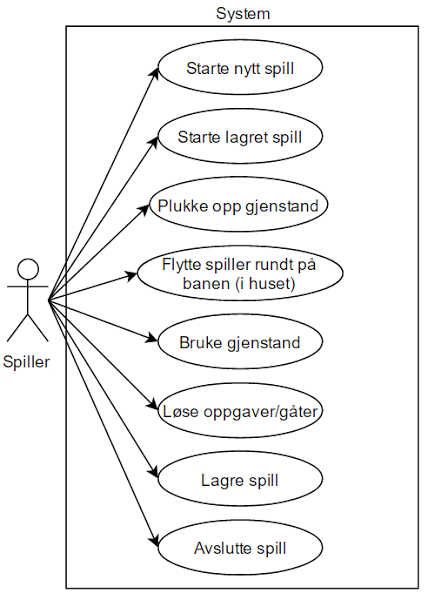
\includegraphics[width=0.8\textwidth,natwidth=500,natheight=642]{use_case_diagram_s.png}

\end{document}